\label{current_research}
Supporting a diverse set of computational campaigns on HPC resources requires the used middleware to be able to support workflows with different computational characteristics.
Scientific applications that are compute-intensive are very well supported by HPC resources.
On the other hand, data-intensive applications do not have the same level of support.
A computational campaign can be comprised either by compute intensive, data intensive or compute and data intensive workflows.
As a result, supporting both types of workflows on HPC resources is important.

\subsection{Data analytics on HPC}
\label{data_analysis_hpc}
Task-parallel frameworks, used mainly for data-intensive applications, involve partitioning a workload into a set of self-contained units of work. 
Based on the application, these tasks can be independent or coupled with varying degrees of data dependencies. 
Scientific workflows exploit task parallelism for simulations as well as data analysis.
Scientific data analysis tools, such as MDAnalysis~\cite{gowers2016mdanalysis,michaud2011mdanalysis}, support domain specific data analytics, but scaling on large data volumes remains a challenge.
These volumes of data are either produced on HPC resources via simulations or acquired via sensors on HPC resources.
As a result, there is a need to support scalable data analytics on the same resources, and especially on HPC resources.

Task-parallel frameworks such as Hadoop~\cite{hadoop}, and Spark~\cite{zaharia2010spark} have been used widely to support scalable data analytics.
There are frameworks for executing and running Hadoop and Spark on HPC resources.
Framework, such as MagPie~\cite{magpie}, JUMMP~\cite{moody2013jummp}, and MyHadoop~\cite{krishnan04myhadoop}, support Hadoop on HPC resources.
These approaches do not support the interoperability of data generation/ acquisition and data analysis that is required.

The Pilot-abstraction~\cite{luckow2012pstar} has been successfully used on HPC resources to support a diverse set of task-parallel applications, via its implementation RADICAL-Pilot~\cite{merzky2019using}.
We extended RADICAL-Pilot to support data-parallel frameworks, such as Hadoop and Spark, on HPC resources~\cite{luckow2016hadoop}.
The extension allows users to execute Hadoop- or Spark-style data analysis on HPC resources.
It is important to note that RADICAL-Pilot is responsible to start, and manage a Hadoop or Spark cluster seamlessly from the user.

We investigated~\cite{paraskevakos2018task} the suitability of task-parallel frameworks for Molecular Dynamics trajectory data analysis. 
The analysis included Spark~\cite{zaharia2010spark}, Dask~\cite{rocklin2015dask}, and RADICAL-Pilot~\cite{merzky2019using}. 
The MD analysis algorithms investigated were selected from MDAnalysis~\cite{gowers2016mdanalysis,michaud2011mdanalysis}. 
The first algorithm is embarrassingly parallel and has no dependencies between tasks, while the second algorithm is a MapReduce algorithm.

\begin{figure*}[t]
    \centering
    \begin{subfigure}[b]{0.45\textwidth}
        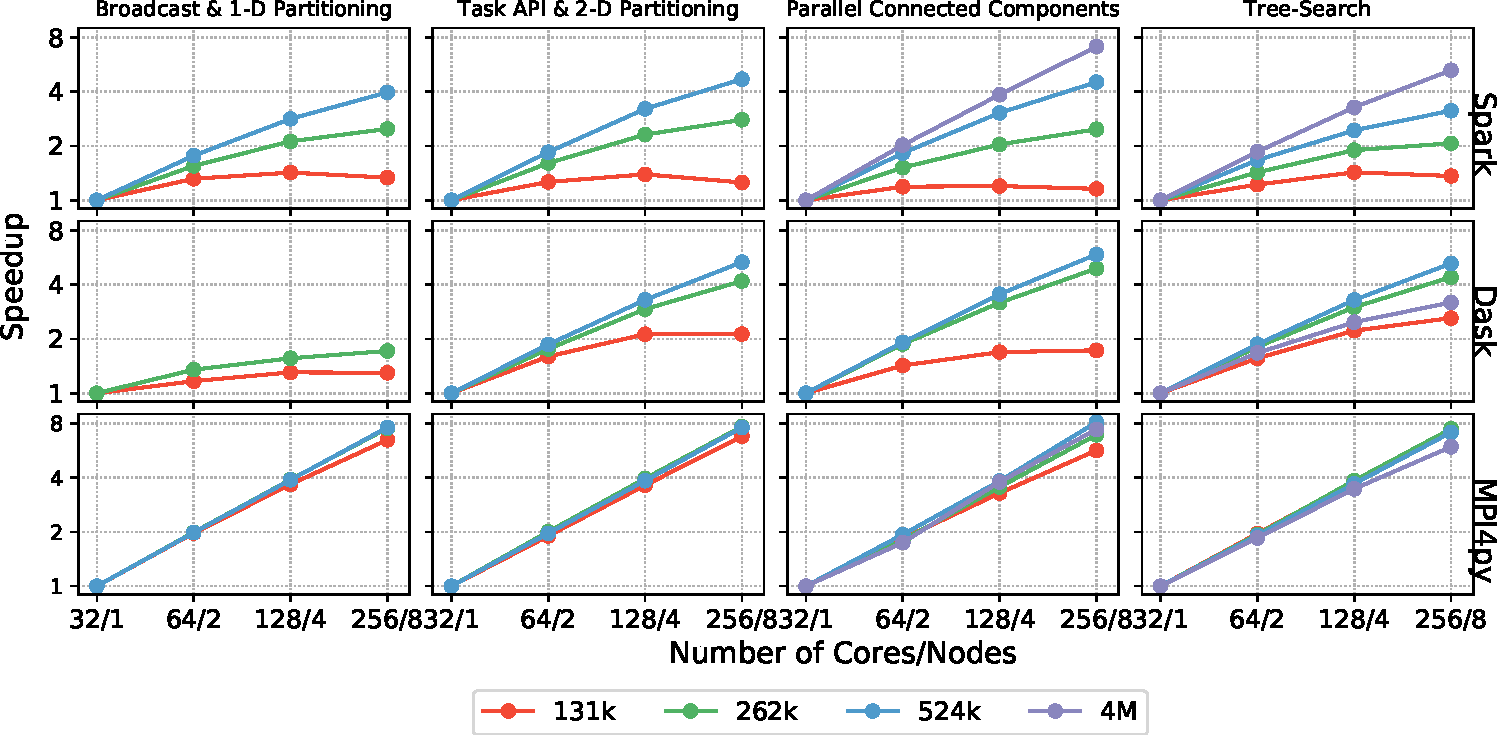
\includegraphics[width=.95\textwidth]{figures/All4approachesWith4MSpeedup.pdf}
        \caption{}
        \label{fig:leafletfinder}
    \end{subfigure}%
    ~ 
    \begin{subfigure}[b]{0.45\textwidth}
        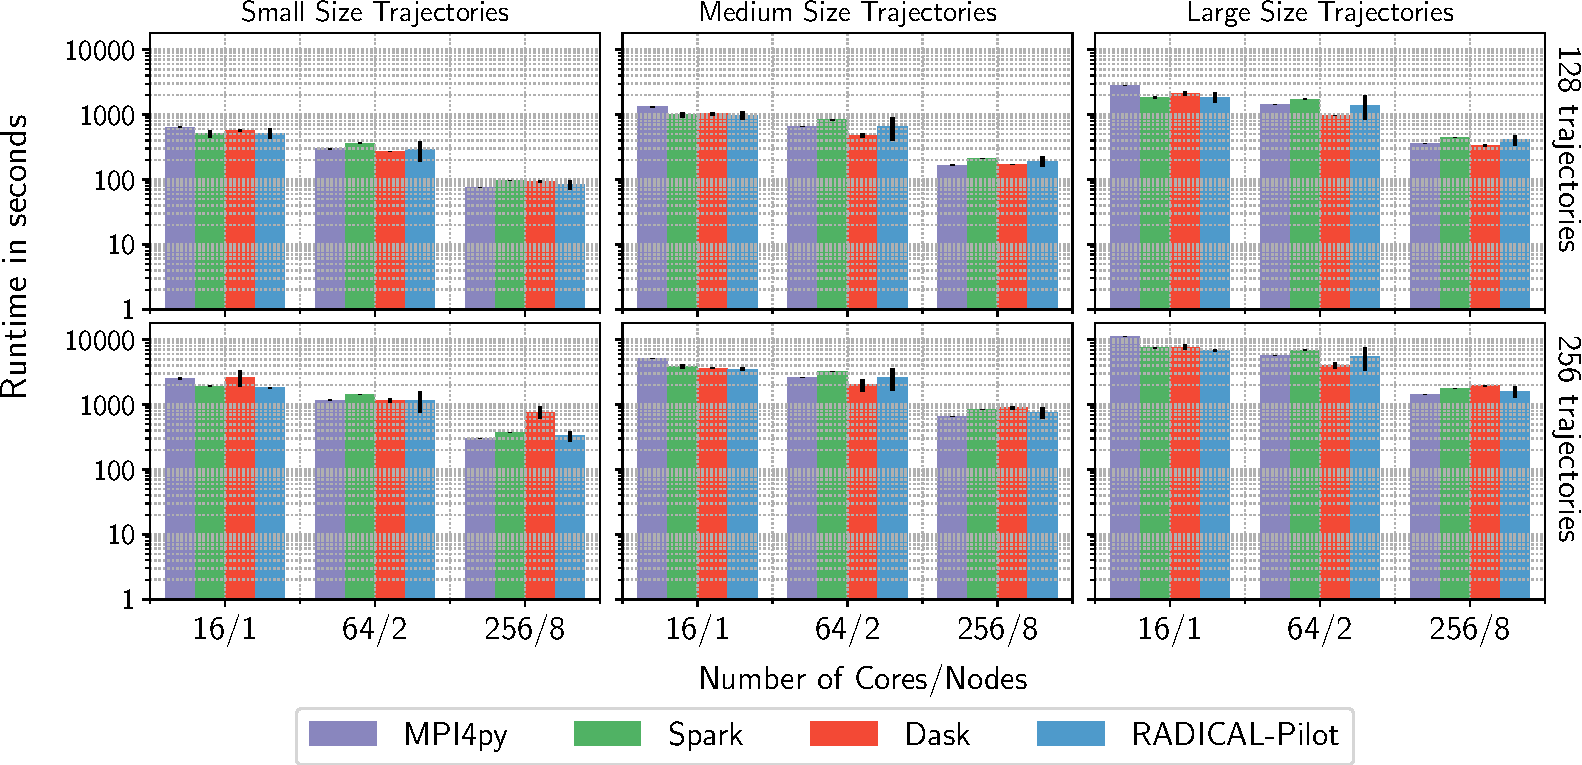
\includegraphics[width=\linewidth]{figures/HausdorffSingleFig.pdf}
        \caption{}
        \label{fig:hausdorff}
    \end{subfigure}
    \caption{~\ref{fig:leafletfinder}Molecular dynamics analysis MapReduce algorithm speedup.~\ref{fig:hausdorff} Molecular dynamics analysis embarrassingly parallel algorithm execution time.}\label{fig:md_analysis}
\end{figure*}

As shown in Figure~\ref{fig:md_analysis}, there are cases where the performance of a parallel implementation is far from ideal, while under different circumstances is as expected. 
For example in Figure~\ref{fig:leafletfinder}, we see that, based on data size Dask provides better speedup than Spark. 
In these cases Dask better utilized the resources compared to Dask, while on others Spark was better.

Implementation aspects, such as computational complexity, and shuffled data size influence the performance greatly. 
For embarrassingly parallel applications with coarse grained tasks the choice of the framework does not significantly influence performance. 
For fine-grained data parallelism, a data-parallel framework is more suited compared to a workload execution framework. 
In addition, the data shuffling size significantly impacts performance and needs to be included in a decision.
The performance analysis of these algorithms implemented in all three frameworks provided us with information to create a conceptual model for selecting the better suitable framework based on algorithmic characteristics.

Data analysis during scientific campaigns may vary depending on the stage of the campaign. 
As a result, the ability to select the best suited framework, given requirements and constraints to execute it is important. 

\subsection{Workflow execution based on middleware design}
\label{design_comp}
Task-parallel data-driven workflow design and execution requires an understanding of the used middleware design, as well as the overheads imposed.
Having a methodology to compare the performance and overheads of different design that in independent of the use case and computing framework becomes important.
We developed experimentally such methodology in Ref.~\cite{paraskevakos2019workflow} using a paradigmatic use case from the earth sciences.

In Ref.~\cite{paraskevakos2019workflow}, we compare the execution time of a data-intensive workflow, as well as the overheads of three different designs that support the use case.
Specifically, the workflow under investigation requires the execution of two tasks consecutively over a set of inputs. 
The tasks are heterogeneous, and have different computational requirements. 
Design 1 implements uses a program-based task parallel framework to execute the workflow, while designs 2 and 2A use a queue based middleware.
Figure~\ref{fig:designs} shows the three designs under comparison, and Fig.~\ref{fig:overall_performance} shows the comparison between the execution time of the workflows per design, and their respective overheads.

\begin{figure*}[ht!]
    \centering
    \begin{subfigure}[b]{0.32\textwidth}
        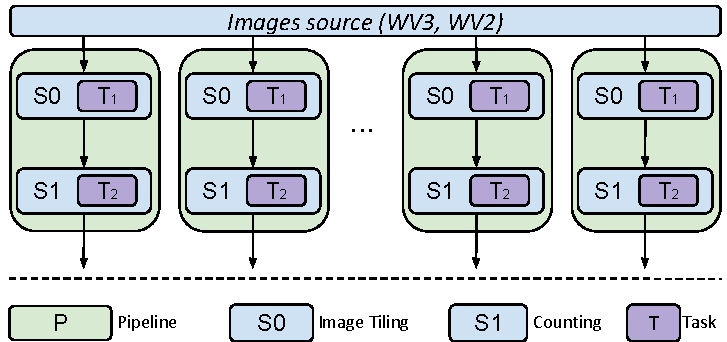
\includegraphics[width=\linewidth]{figures/SealsDesign1.pdf}
        \caption{}
		\label{fig:seals_design1}
    \end{subfigure}%
    ~ 
    \begin{subfigure}[b]{0.32\textwidth}
        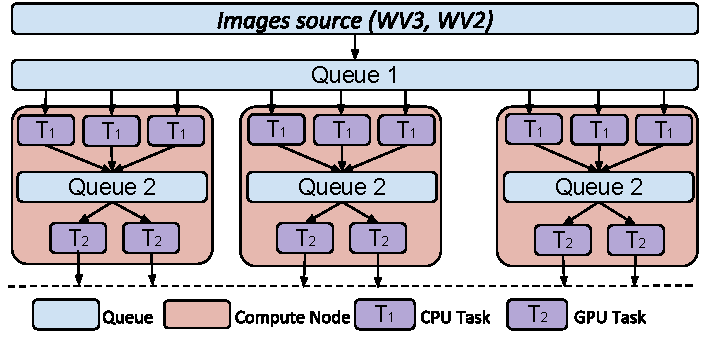
\includegraphics[width=\linewidth]{figures/SealsDesign2.pdf}
        \caption{}\label{fig:seals_design2}
    \end{subfigure}%
    ~ 
    \begin{subfigure}[b]{0.32\textwidth}
        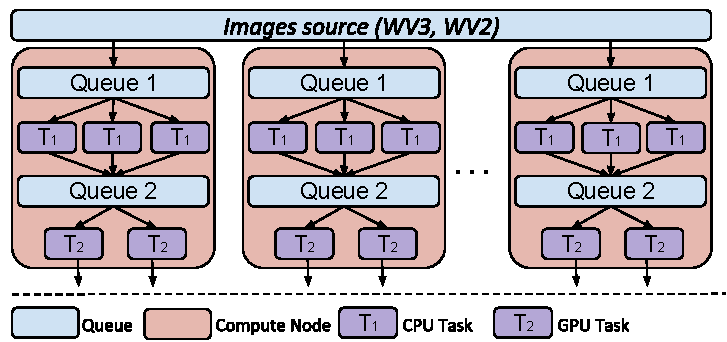
\includegraphics[width=\linewidth]{figures/SealsDesign3.pdf}
		\caption{}\label{fig:seals_design3}
    \end{subfigure}
    \caption{Design approaches to implement the workflow required for the
    Seals use case.~\ref{fig:seals_design1}--\textbf{Design 1}: Pipeline,
    stage and task based design.~\ref{fig:seals_design2}--\textbf{Design 2}:
    Queue based design with a single queue for all the tiling
    tasks.~\ref{fig:seals_design3}--\textbf{Design 2.A}: Queue based design
    with multiple queues for the tiling tasks.}\label{fig:designs}
\end{figure*}

Figure~\ref{fig:ttx} shows the execution time of different designs that support the use case. 
The execution time between designs 1 and 2 are within error bars.
Figure~\ref{fig:overheads} shows the overheads imposed by each design.
Design 2A shows the best performance in terms of overheads, and execution time.
Design 2 shows similar overheads, but it showed worse execution time compared to design 2A.
Design 1 shows imposes the most overheads, due to executing a program for each task of the workflow, imposing bootstrap and tear down overheads.

\begin{figure*}[ht!]
    \centering
    \begin{subfigure}[b]{0.45\textwidth}
        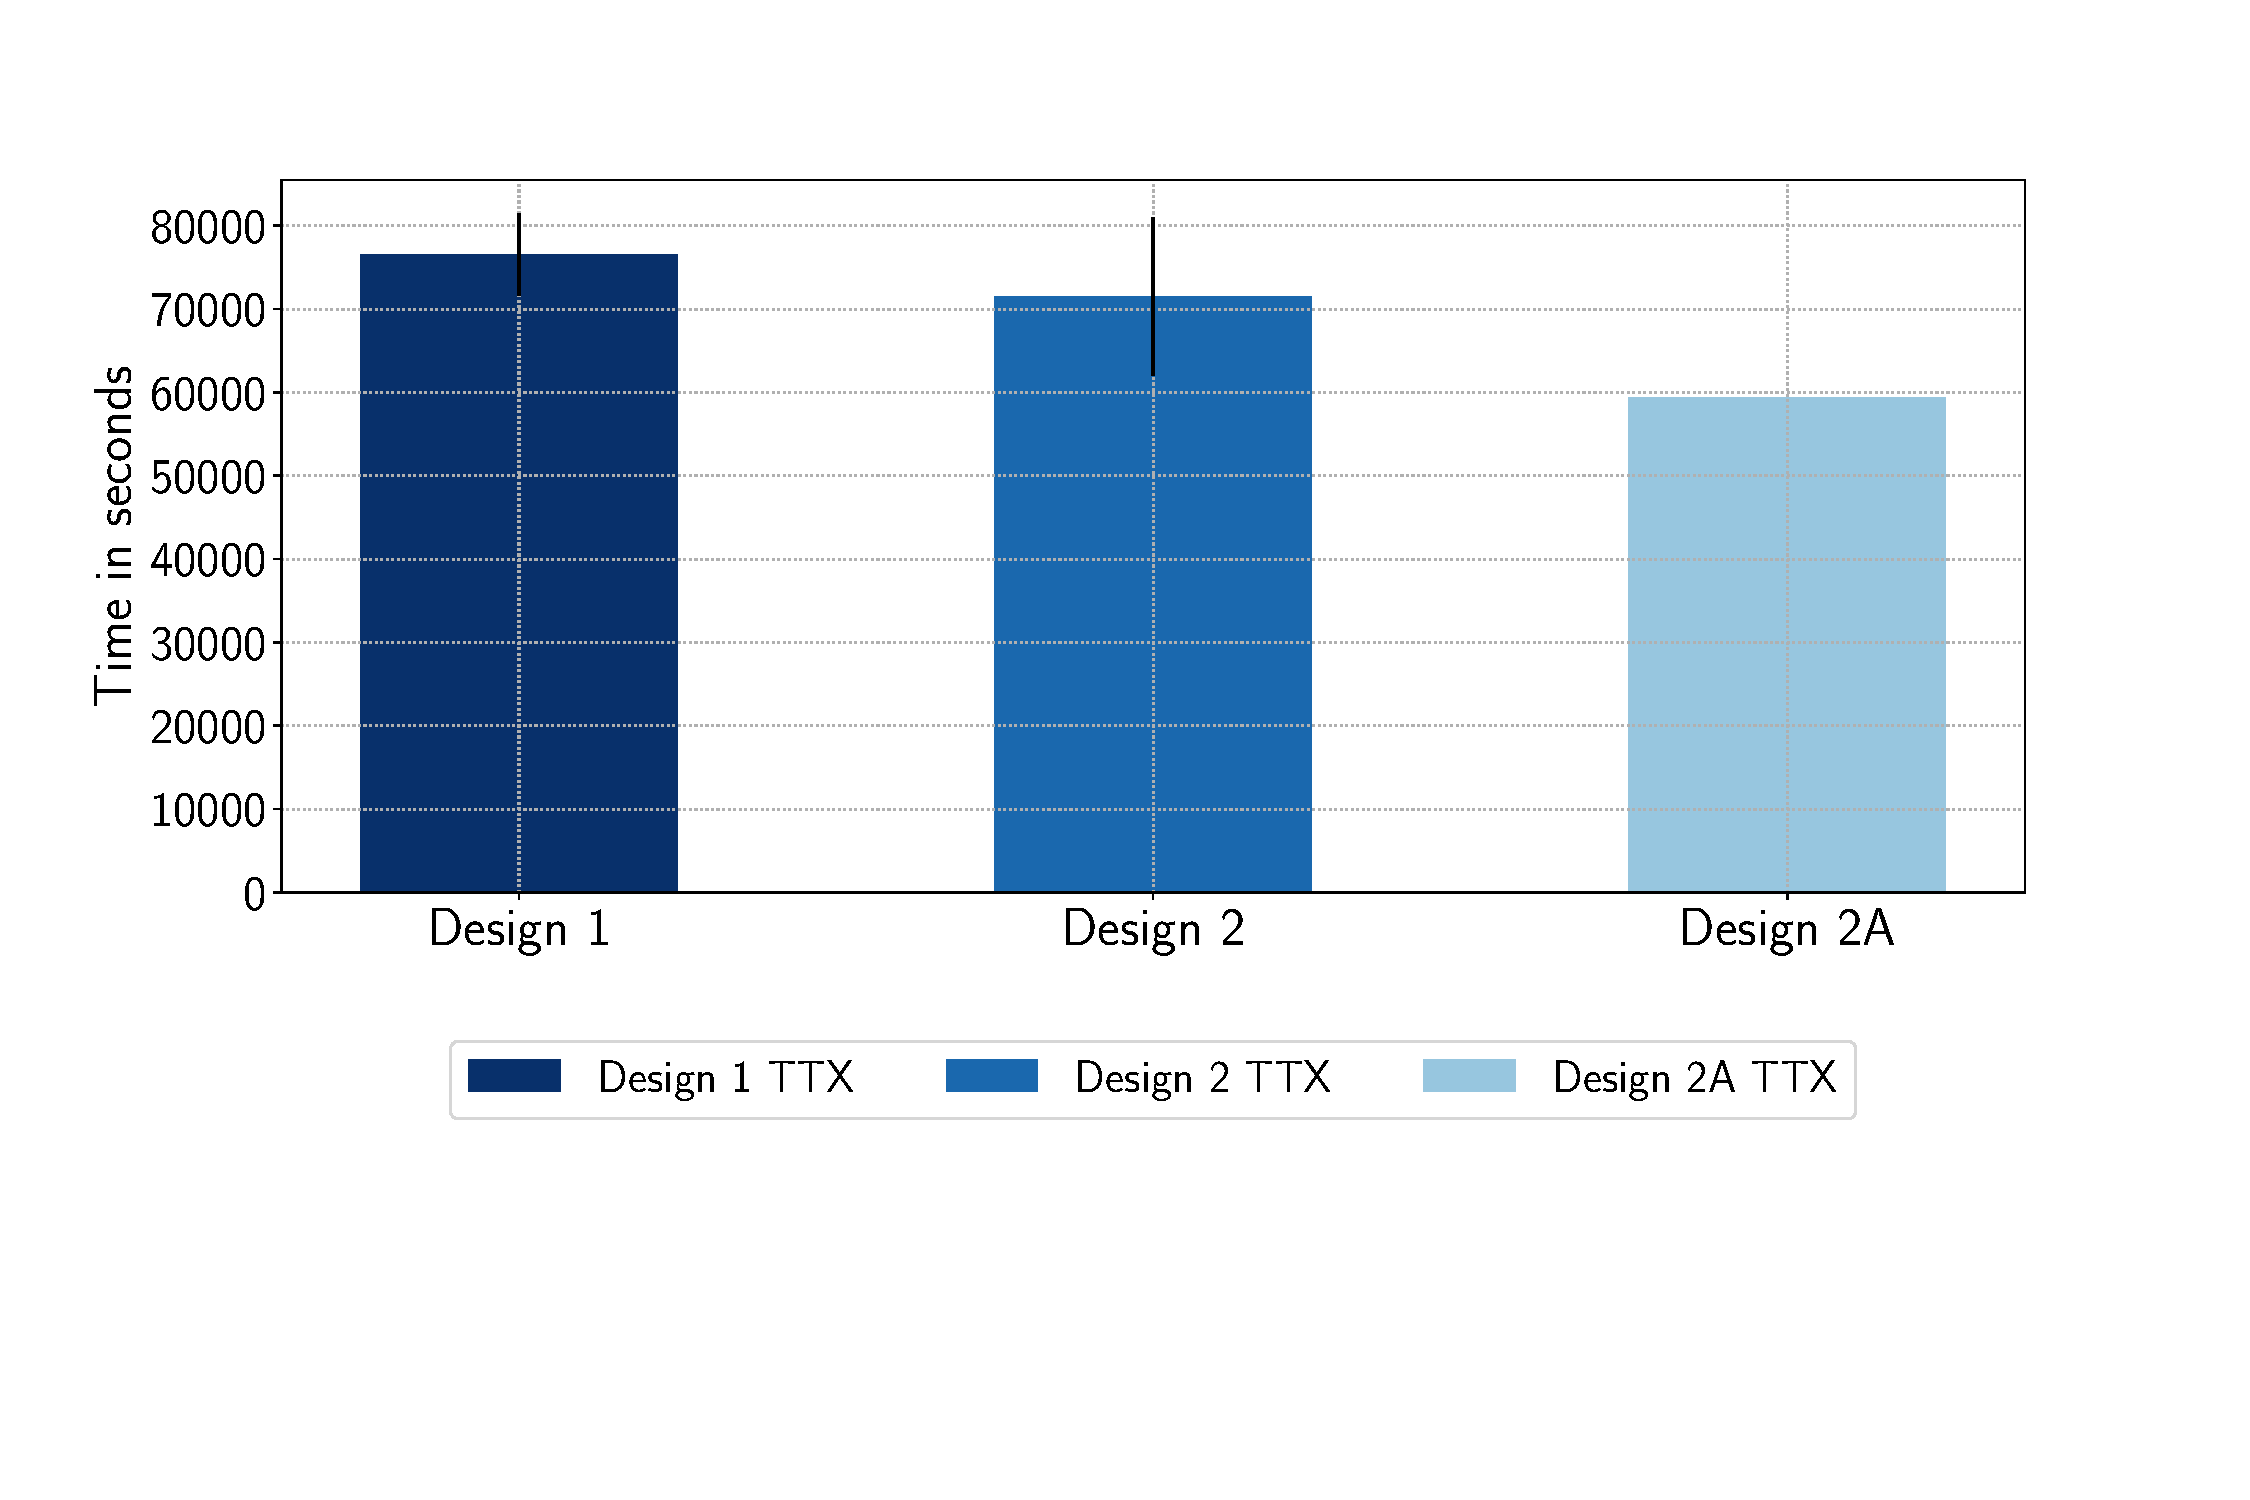
\includegraphics[width=\linewidth]{figures/ttx.pdf}
        \caption{}
        \label{fig:ttx}
    \end{subfigure}%
    ~ 
    \begin{subfigure}[b]{0.45\textwidth}
        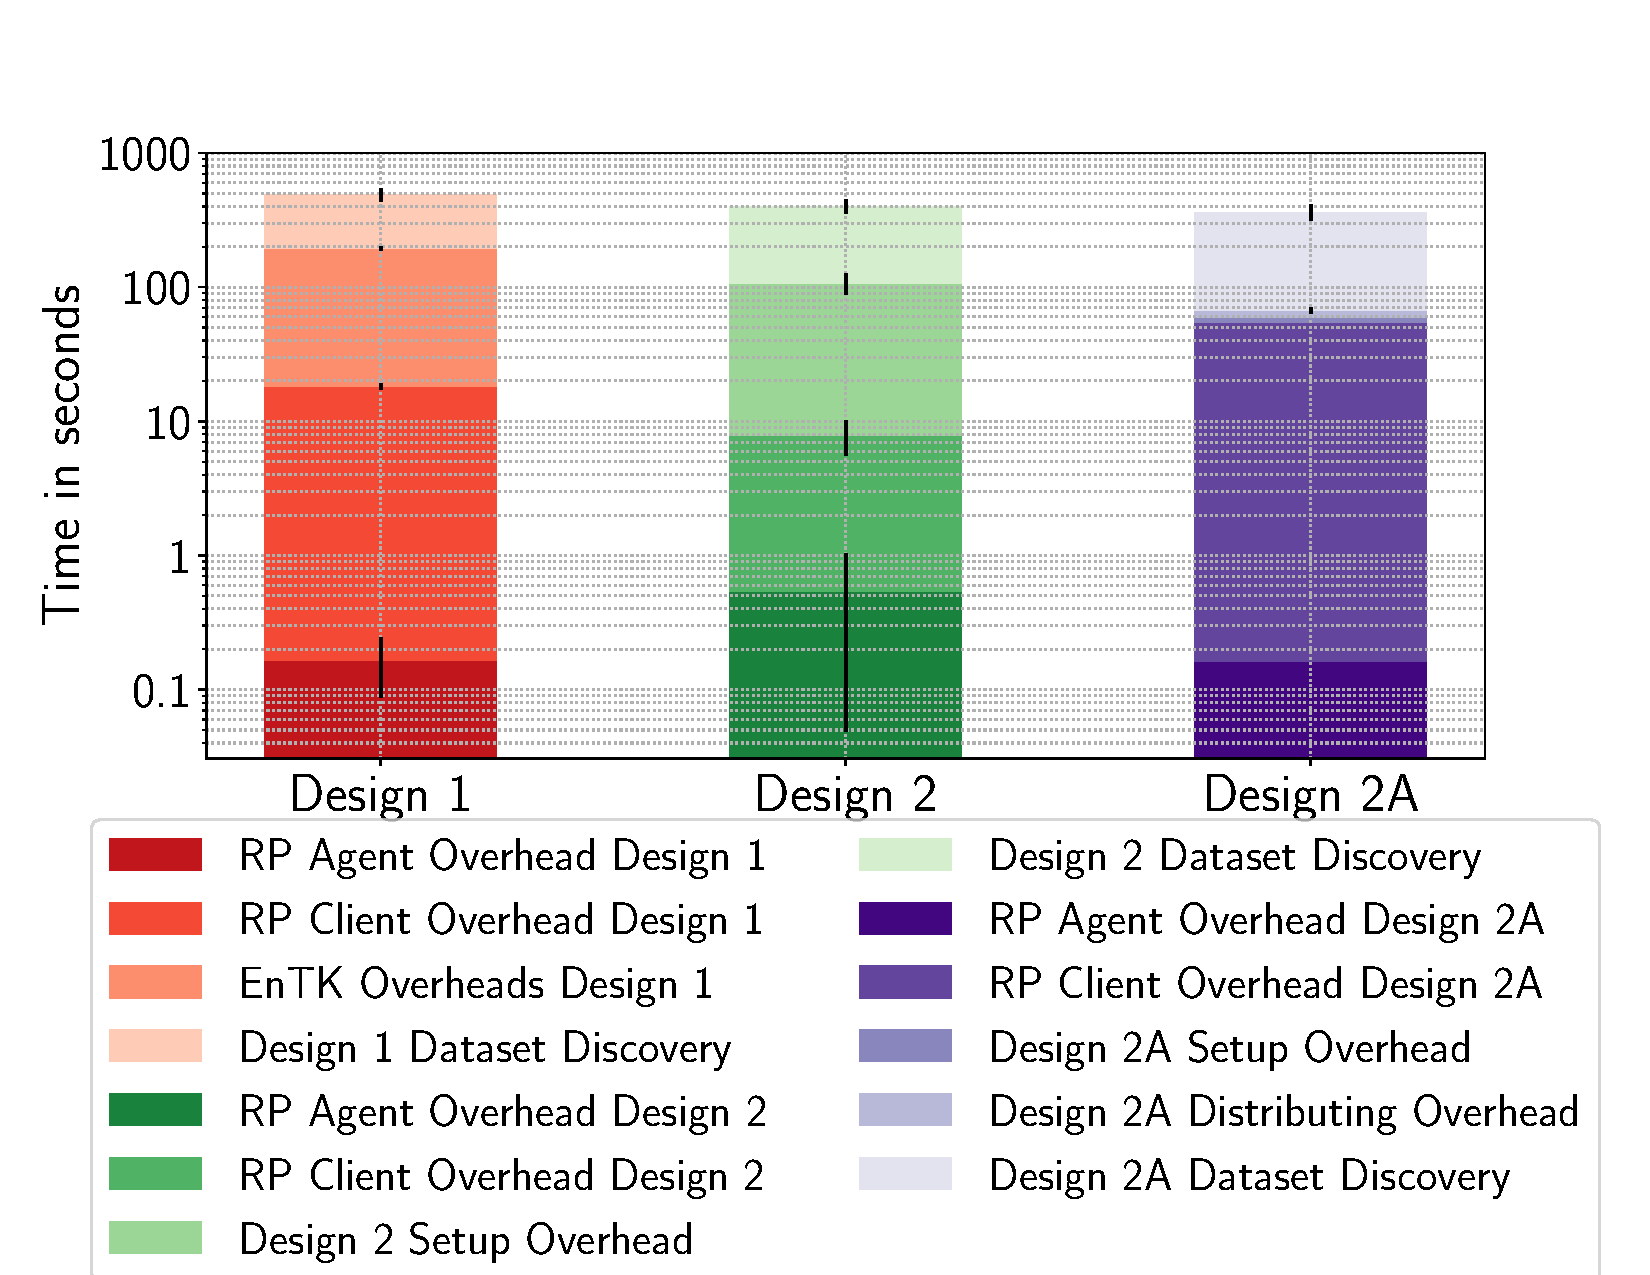
\includegraphics[width=\linewidth]{figures/overheads.pdf}
        \caption{}
        \label{fig:overheads}
    \end{subfigure}
    \caption{~\ref{fig:ttx} Total execution time of Design~1, 2 and 2.A. Design~1 and 2 have similar performance, Design~2.A is the fastest. ~\ref{fig:overheads} Overheads of Design~1, 2 and 2.A are at least two orders of magnitude less than the total execution time.}\label{fig:overall_performance}
\end{figure*}

Our experiment based methodology to compare designs applies to the evaluation of designs of existing and future computing frameworks to support data-intensive workflows.
We can use the overheads characterization as a baseline to evaluate a production-grade implementations, as well as identify the bottlenecks of the used middleware.




\subsection{Related Work}
% ----------------------------------------------------------------------------
% Campaign management system
\gpnote{write about Panda, Blasam, Pegasus, ASKALON, DIRAC, QCFractal(?), GlideInWMS}

There are software systems that are supporting computational campaigns in one way or another. 
PanDA WMS~\cite{maeno2008panda,maeno2014evolution}, possibly the most widely used workload and workflow management system, DIRAC~\cite{casajus2010dirac}, and glideinWMS~\cite{sfiligoi2008glidein} support domain specific workflows.
These systems assume a specific software stack environment that support their use case.
Our approach is domain agnostic and it makes zero assumptions of a specific pre-existing software stack. 
Furthermore, PanDA, DIRAC, and glideIN are grid oriented campaign managers, without or minimal support of HPC resources.
For example, PanDA undergoes an effort to support HPC~\cite{de2016accelerating}, but it is limited to ORNL Titan~\cite{titan}.
Workflow management systems on HPCs, like Pegasus~\cite{deelman2015pegasus}, and Balsam~\cite{salim2019balsam} support the execution of multiple workflows on HPC resources from multiple users as independent entities.
A common denominator between all the above campaign, workflow or workload managers, is that they provide a capability to define a set of workflows with a common computational objective.
We want to extend this notion and allow users to define a single computational objective for a campaign.
As a result, the above execution model becomes a special case, where a campaign is a single workflow.